\documentclass[final,hyperref={pdfpagelabels=false}]{beamer}
\usepackage{grffile}
\mode<presentation>{\usetheme{I6pd2}}
\usepackage[english]{babel}
\usepackage[utf8]{inputenc}
\usepackage{gensymb}
\usepackage{amsmath,amsthm, amssymb, latexsym}
%\usepackage{times}\usefonttheme{professionalfonts}  % obsolete
%\usefonttheme[onlymath]{serif}
\boldmath
\usepackage[orientation=portrait,size=a0,scale=1.4,debug]{beamerposter}
% change list indention level
% \setdefaultleftmargin{3em}{}{}{}{}{}

\usepackage{multicol}
%\usepackage{snapshot} % will write a .dep file with all dependencies, allows for easy bundling

\usepackage{array,booktabs,tabularx}
\newcolumntype{Z}{>{\centering\arraybackslash}X} % centered tabularx columns
\newcommand{\pphantom}{\textcolor{ta3aluminium}} % phantom introduces a vertical space in p formatted table columns??!!

\listfiles

%%%%%%%%%%%%%%%%%%%%%%%%%%%%%%%%%%%%%%%%%%%%%%%%%%%%%%%%%%%%%%%%%%%%%%%%%%%%%%%%%%%%%%
\graphicspath{{figures/}}

\setlogo{figures/logo_ghd}
\setauthorurl{http://geohistoricaldata.org}
\setauthoremail{contact@geohistoricaldata.org}

\title{A roadmap for a reproducible approach to geo-historical information\\from its capture to its analysis}
\author{GeoHistoricalData}
\institute{~}
\date{October 2018}
%%%%%%%%%%%%%%%%%%%%%%%%%%%%%%%%%%%%%%%%%%%%%%%%%%%%%%%%%%%%%%%%%%%%%%%%%%%%%%%%%%%%%%
\newlength{\columnheight}
\setlength{\columnheight}{105cm}

\hypersetup{colorlinks,linkcolor=,urlcolor=ta3skyblue}
\let\oldcite=\cite
\renewcommand{\cite}[1]{\textcolor{ta3chameleon}{\oldcite{#1}}}
%% \usepackage{enumitem}
%% \setlist[description]{%
%%   topsep=0pt,               % space before start / after end of list
%%   itemsep=0pt,               % space between items
%%   font={\bfseries\sffamily\tiny\color{ta3orange}}, % set the label font
%% %  font={\bfseries\sffamily\color{red}}, % if colour is needed
%% }
\usepackage{calc}
\makeatletter
\def\Mdescription#1{%
  \advance\beamer@descdefault by \labelsep%
  \list
  {}
  {\labelwidth\beamer@descdefault%
  \leftmargin\beamer@descdefault%
  \let\makelabel\beamer@descriptionitem
  \settowidth\labelwidth{\beamer@descriptionitem{#1}}%
  \setlength\leftmargin{\labelwidth}% 
  \addtolength\leftmargin{\labelsep}%
  }%
  \beamer@cramped%
  \raggedright
  \beamer@firstlineitemizeunskip%
}
\def\endMdescription{\ifhmode\unskip\fi\endlist}
\long\def\beamer@descriptionitem#1{%
  \def\insertdescriptionitem{#1}%
  {\usebeamertemplate**{description item}}\hfil}
\makeatother
%%%%%%%%%%%%%%%%%%%%%%%%%%%%%%%%%%%%%%%%%%%%%%%%%%%%%%%%%%%%%%%%%%%%%%%%%%%%%%%%%%%%%%

\begin{document}

\begin{frame}
  \begin{block}{What is the GeoHistoricalData Project?}
    \textcolor{ta3orange}{GeoHistoricalData} (GHD) is a long-term collaborative research project involving researchers from several institutions (EHESS, IGN, National Archives, EPITA, etc.).\\
    In addition to a methodological approach to the construction of geo-historical information, we also promote research in collaboration with other research groups focused on specific territories and time periods:
    %\text{Vectorisation collaborative : Sur l'ensemble du territoire Français: Une série d'images montrant les progrès de la saisie des routes ??? / Carte des clochers ??? / allignement avec avec la base des communes 1793-2006}\\
    \begin{itemize}
    \item \textcolor{blue}{Metropolitan France:} \textcolor{ta3orange}{Cassini} map thematic vectorisation (roads, churches, etc.)
    \item \textcolor{blue}{Auvergne:} \textcolor{ta3orange}{reconstruction of Cassini sheet n$^{o}$52} with the University of Clermont-Ferrand
      %\text{Vectorisation collaborative approche locale (Clermont) : reconstitution numérique de la planche 52 originale / analyse des proximités des lieux habités de la planche }\\
    \item \textcolor{blue}{Paris:} spatio-temporal databases and geocoding, including \textcolor{ta3orange}{St Jean de Latran}~\cite{Rebolledo-Dhuin2014}
%      \text{Paris : base de données spatio-temporelle / geocodage automatisé }\\
      %    Dossier St Jean de Latran (\cite{Rebolledo-Dhuin2014})\\
    \end{itemize}
  \end{block}
  \begin{columns}
    \begin{column}{0.5\textwidth}
    \begin{beamercolorbox}[center,wd=\textwidth]{postercolumn}
    \begin{minipage}[t]{.98\textwidth}
    \renewcommand{\footnoterule}{}
    \begin{block}{Primary Sources and Georeferencing}
      \centering
      \begin{tabular}{p{0.45\textwidth}p{0.45\textwidth}}
        \multicolumn{2}{p{0.9\textwidth}}{Beyond the georeferencing and the digitization of the maps, we also propose a thourough analysis of these maps, including their planimetric accuracy (See \cite{Dumenieu2013a,Dumenieu2015PhD,Dumenieu2018}).}\\
        \multicolumn{2}{c}{\includegraphics[width=0.8\textwidth,trim={0 4cm 0 2cm},clip]{figures/plans_V2.png}}\\
	\multicolumn{2}{c}{\scriptsize Sample maps of Paris}\\%ajouter par ici les "temps valides" des cartes.
        \multicolumn{2}{p{0.9\textwidth}}{
          \tiny{
            \textsc{\textbf{Verniquet 1784-1791}:}
            \textit{Atlas du plan général de la ville de Paris, levé géométriquement par le cen \textsc{Verniquet} rapporté sur une échelle d'une demie ligne pour toise}, divisée en 72 planches, compris les cartouches et plan des opérations trigonométriques.
            Dessiné et gravé par les cens \textsc{Bartholomé} et \textsc{Mathieu}...,
            Se trouve à Paris: chez l'auteur, rue de l'Oratoire, n 146, (an \textsc{iv} [1795]), gr. in-fol. plano de 71 pl. ;
            \textsc{\textbf{Vasserot 1808-1836}:}
            \textit{Atlas général des quarante-huit quartiers de la ville de Paris}, dressé et publié par Ph. \textsc{Vasserot},... et I.-G. \textsc{Bellanger},..., [S. l.], [s. n.], [s. d.], gr. in-fol de 83 pl. ;
            \textsc{\textbf{Jacoubet 1827-1836}:}
            \textit{Atlas général de la ville, des faubourgs et des monuments de Paris} par Th. \textsc{Jacoubet},..., (S. l.,), 1836, Gr. in-fol., carte en 52 pl. and \textit{Atlas municipal des vingt arrondissements de la ville de Paris}, dressé sous l'administration de M. E.
            \textsc{\textbf{Alphand 1888}:}\textsc{Poubelle} préfet, sous la direction de M. \textsc{Alphand}...; par les soins de M. L. \textsc{Fauve} géomètre en chef, avec le concours des gémoètres du plan de Paris, [Paris], [L. Wuhrer], 1895, 1 vol., ([1]-16 pl.)
          }
        }\\
	
        \multicolumn{2}{c}{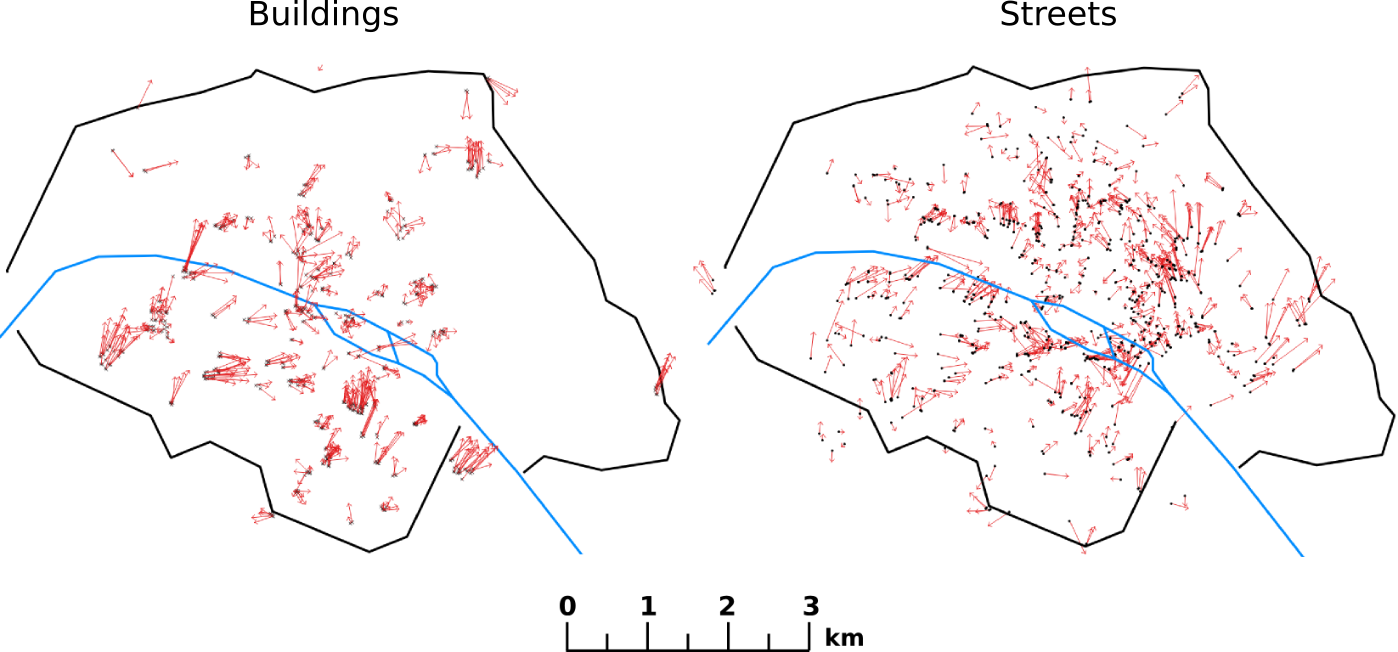
\includegraphics[width=0.6\textwidth]{figures/errorthemes.png}}\\
	\multicolumn{2}{c}{\scriptsize Error vectors measured on street corners and buildings (exaggerated 100 times)}\\
        \vspace{0pt}
        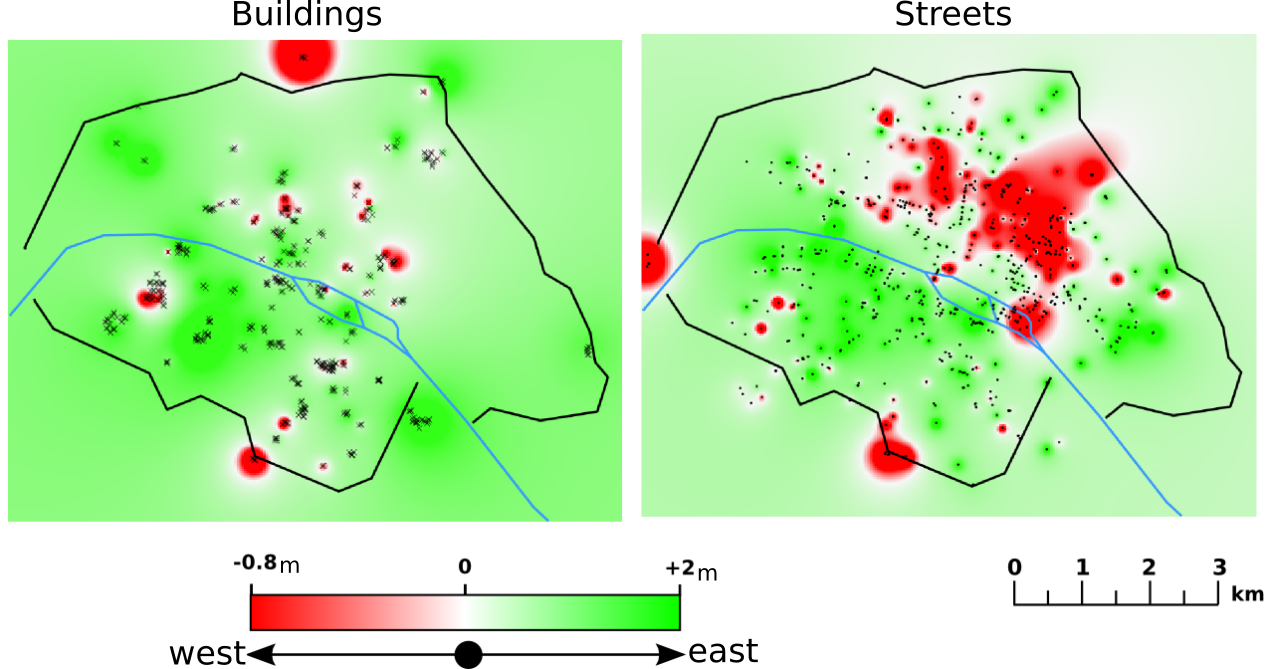
\includegraphics[width=0.4\textwidth]{figures/error_x.png}&
        \vspace{0pt}
        \hspace*{-1em}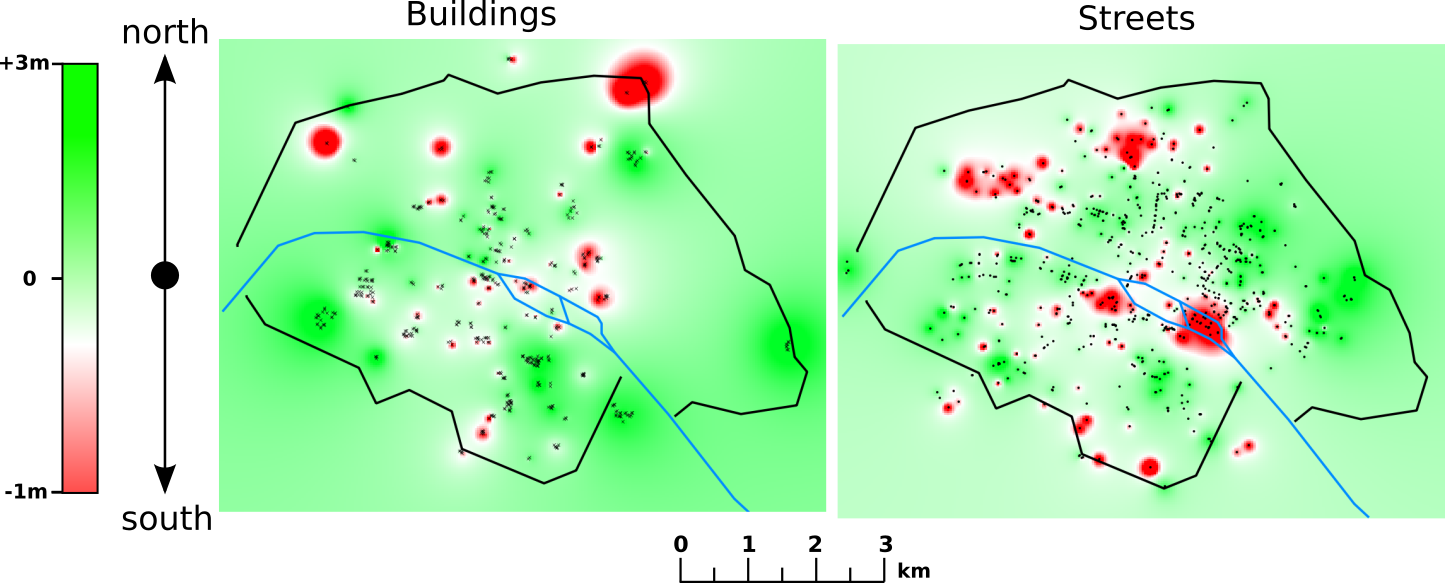
\includegraphics[width=0.48\textwidth]{figures/error_y.png}\\
	\scriptsize Mapping the horizontal component of the distortion vectors&
        \scriptsize Mapping the vertical component of the distortion vectors
      \end{tabular}
    \end{block}
    \begin{block}{Large Historical Geocoding}
      \begin{tabular}{>{\centering}m{0.9\textwidth}}
        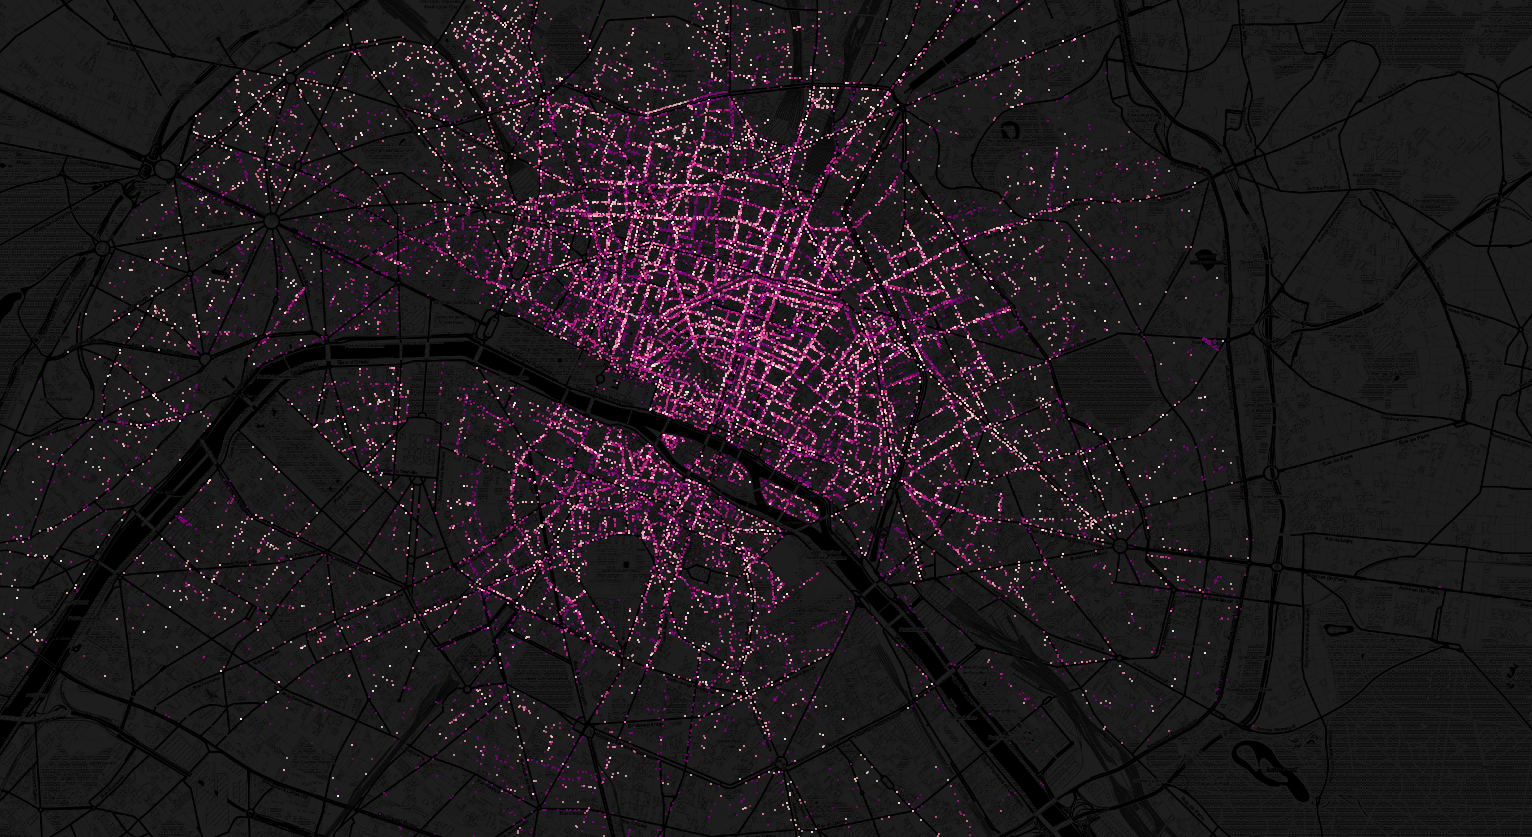
\includegraphics[width=0.65\textwidth]{figures/geocoding}\\
        \scriptsize Sample of geocoded INPI (French National Industrial Property Institute) patents (from \url{http://bases-brevets19e.inpi.fr/}) using the historical geocoder~\cite{Cura2018}
      \end{tabular}
    \end{block}
    \end{minipage}
    \end{beamercolorbox}
    \end{column}
    \begin{column}{0.5\textwidth}
    \begin{beamercolorbox}[center,wd=\textwidth]{postercolumn}
    \begin{minipage}[t]{.98\textwidth}
      \begin{block}{Collaborative Content Extraction}
        \centering
        Topography, natural graphs \textit{\&} historical networks
        \begin{tabular}{>{\centering}p{0.95\textwidth}}
	  \includegraphics[width=0.8\textwidth]{figures/cassini} \\
          \scriptsize Complete collaborative digitization of \tiny{
\textit{Carte générale} \& particulière de la France. N\degree 52. F.\textsuperscript{le} 110 [Clermont en Auvergne]. Carte en couleur de 610 x 955 mm (format « grand-aigle ») à l'échelle 1:86~400 ou 1 ligne pour 100 toises. \textbf{Établie de 1759 à 1777 sous la direction de} César François \textsc{Cassini de Thury}, Charles Étienne Louis \textsc{Camus} (puis Rodolphe \textsc{Perronet}) et d’Étienne \textsc{Mignot de Montigny}. \textbf{Levés de 1759 à 1775} par P. de \textsc{La Court} (\textsc{ne} partiel, 1759), François \textsc{Pasumot}, Claude \textsc{Pezet}, \textsc{Dallier} et \textsc{Dailley} (\textsc{no-so}, c.1764-1766), Louis \textsc{Le Bel} (\textsc{se}, 1766-1768; \textsc{ne} et \textsc{so}, 1769), \textsc{Dubois} \textit{\&} Louis \textsc{Cabay} (\textsc{no-ne}, 1772-1773), \textsc{Querry} \textit{\&} François \textsc{La Ruelle} (\textsc{ne}, 1774-1775). \textbf{Vérifiées sur le terrain, de 1767 à 1774} par P. \textsc{Renault} (\textsc{se}, 1767-1768), \textsc{Querry} \textit{\&} F. \textsc{La Ruelle} (\textsc{no-ne-so}, 1774). \textbf{Gravée à Paris en 1774-1777} par Louis \textsc{Capitaine} fils (pour le plan, 1774-1776) et Nicolas \textsc{Bourgoin} (pour la lettre, 1775-1777). Imprimée en taille-douce sur la presse de l'Observatoire de Paris en 1777 pour le compte de la Compagnie associée pour la Carte générale de la France. Présentée au Roi et la cour royale, à Versailles, le 16 avril 1777 (impression sur « satin »).
})\
        \end{tabular}
        \begin{tabular}{>{\centering}p{0.95\textwidth}}
          \includegraphics[width=0.95\textwidth]{figures/progression}\\
          \scriptsize Progress of the digitization during the first years (in \textcolor{red}{red}: elements digitized during the time period)
        \end{tabular}
      \end{block}
      \begin{block}{Spatial \& Morphological Analysis}
        \centering
	\begin{tabular}{>{\centering}m{0.9\textwidth}}
	  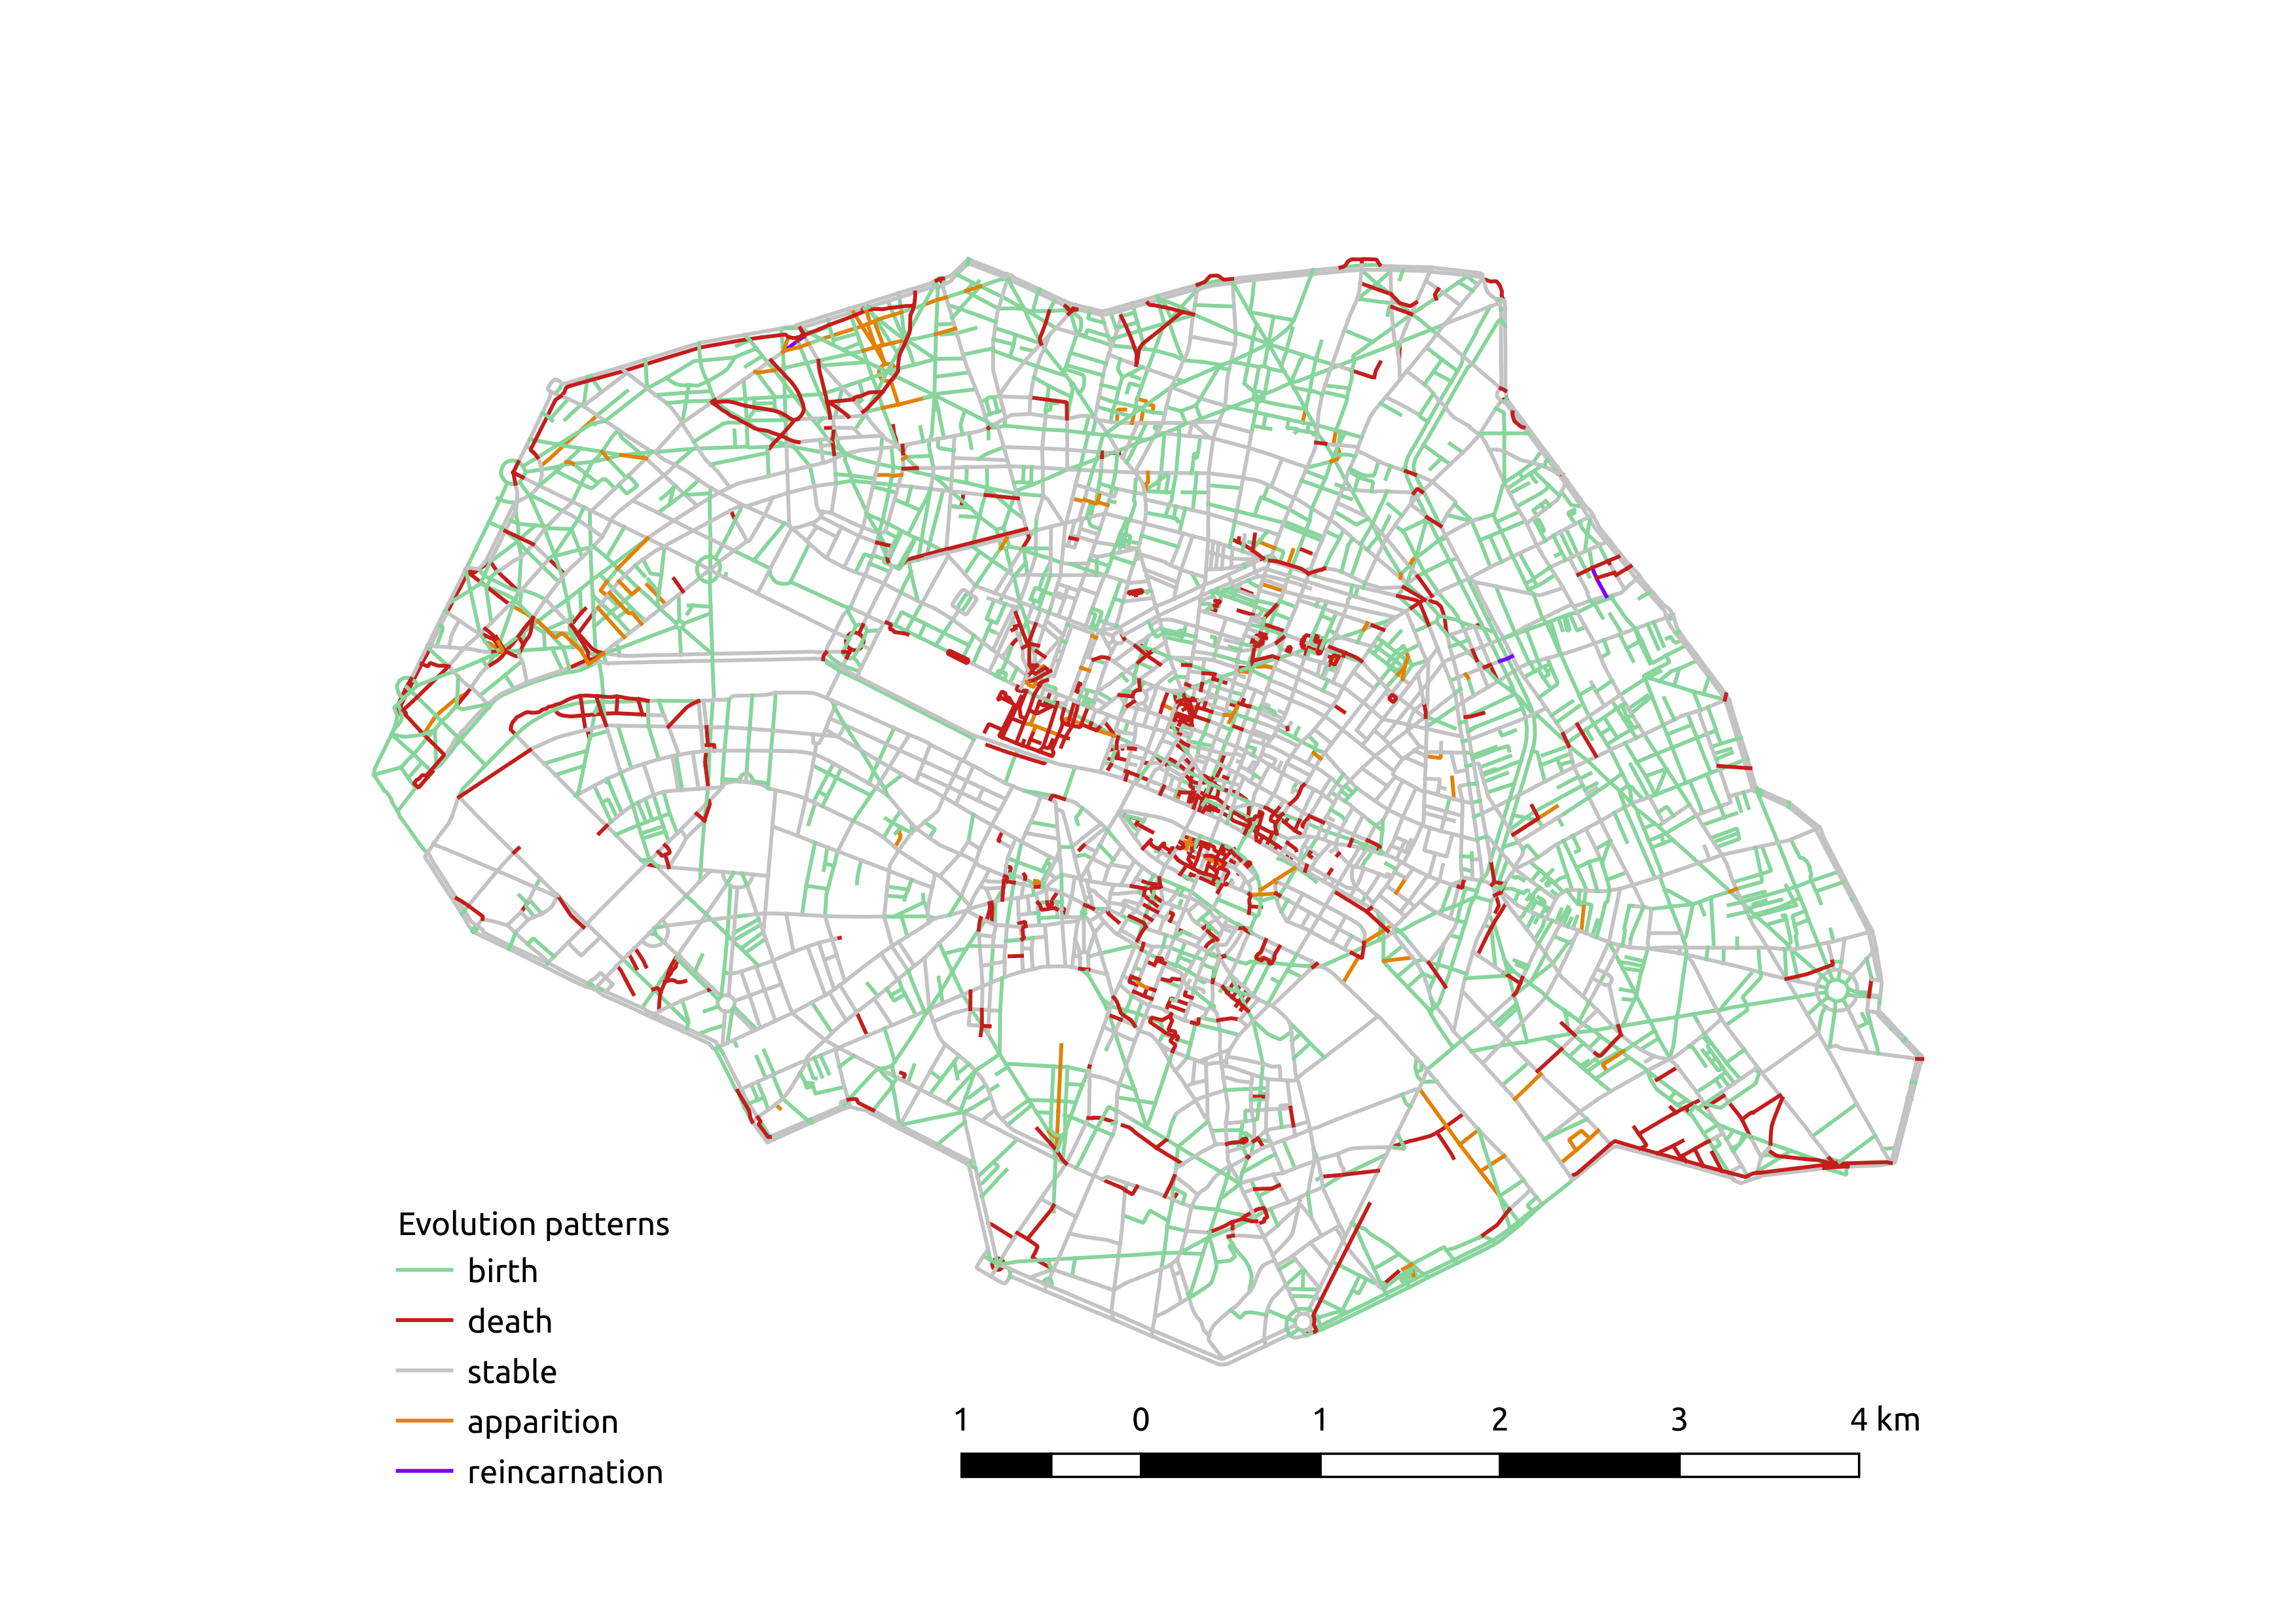
\includegraphics[width=0.5\textwidth,trim={3.5cm 1.25cm 3.5cm 2.5cm},clip]{figures/EvolutionPatterns}\\
	  \scriptsize Example of patterns extracted from the integration of several street networks (see~\cite{Costes2015_,Costes2016PhD})\\
        \end{tabular}
        
        
        \begin{tabular}{>{\centering}m{0.95\textwidth}}
	  
	  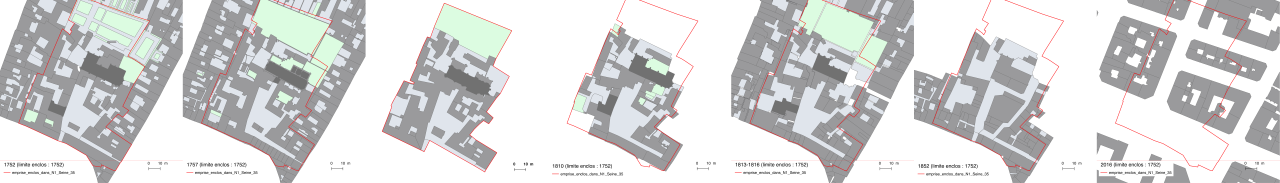
\includegraphics[width=0.9\textwidth]{figures/Latran_1752-2016}\\
	  \scriptsize Saint-Jean-de-Latran, from enclosure to its destruction\\
	  \scriptsize Morphological evolution of a Parisian downtown block (1752-1850, 2016)\\
	  (see~\cite{Rebolledo-Dhuin2014}, from~\url{https://goo.gl/sT3oYw})
        \end{tabular}
        
      \end{block}
    \end{minipage}
    \end{beamercolorbox}
    \end{column}
  \end{columns}
  \begin{columns}
    \begin{column}{0.6\textwidth}
    \begin{beamercolorbox}[center,wd=\textwidth]{postercolumn}
    \begin{minipage}[t]{.98\textwidth}
      \begin{block}{Main contributions}%Conclusion \& Applications}
        \tiny
        %    Our main contributions involve
        \begin{itemize}
        \item a \textcolor{ta3orange}{global approach} to study the co-evolution of spatial and social dynamics~\cite{Dumenieu2013a, Dumenieu2015PhD}
        \item a \textcolor{ta3orange}{critical analysis} of \textcolor{ta3orange}{primary sources}~\cite{Costes2015_, Dumenieu2015PhD, Costes2016PhD, Dumenieu2018}
        \item the \textcolor{ta3orange}{collaborative co-construction} of geo-historical information~\cite{Perret2015_, Perret2015Data_, Cura2018}
        \end{itemize}
      \end{block}
    \end{minipage}
    \end{beamercolorbox}
    \end{column}
    \begin{column}{0.4\textwidth}
      \begin{beamercolorbox}[center,wd=\textwidth]{postercolumn}
        \begin{minipage}[t]{.98\textwidth}
          \begin{block}{Open science}
            %\setbeamertemplate{description item}[align left]
            \begin{Mdescription}{Grouppp}
              \tiny
              %Website: \url{http://geohistoricaldata.org/}\\
            \item[\textcolor{ta3orange}{Group:}] \url{https://github.com/GeoHistoricalData}\\
            \item[\textcolor{ta3orange}{Geocoder:}] \url{https://github.com/GeoHistoricalData/historical_geocoding}\\
            \item[\textcolor{ta3orange}{Datasets:}]
              \begin{itemize}\tiny
              \item The 18$^{th}$ century Cassini roads and cities dataset: \url{https://dataverse.harvard.edu/dataset.xhtml?persistentId=doi:10.7910/DVN/28674}\\
              \item Other datasets are available from the website.
              \end{itemize}
            \item[\textcolor{ta3orange}{Semantic Wiki:}] \url{http://wiki.geohistoricaldata.org/}
            \end{Mdescription}
          \end{block}
        \end{minipage}
      \end{beamercolorbox}
    \end{column}
  \end{columns}
  
  \begin{block}{References}
    \vspace*{-1.5em}
	\begin{multicols}{2}
		\tiny
		\bibliographystyle{alpha}
		\bibliography{main}
	\end{multicols}
  \end{block}
\end{frame}
\end{document}

